\section{Finite Element Method}
\label{s.fem}

In this section, we present the main concepts related to the Finite Element Method. Broadly speaking, FEM aims at approximating functions given a set of sampled points by means of basis functions. In a first step, the basis functions are used to interpolate the manifold based on the sampled points (domain) and their respective responses to that functions (image). Further, the approximation step aims at interpolating new points to the learned manifold.

\subsection{Function Approximation}
\label{ss.function}

Let ${\cal D}$ and ${\cal V}$ be an infinite and a non-trivial set, respectively, and $F:{\cal D}\rightarrow{\cal V}$ be a function that contains an infinite number of mappings. Therefore, $F$ can not be represented as a generic element in computers, and thus one needs to replace $F$ by an approximation function $\tilde{F}$ in some finite subspace. Additionally, the quality of the approximation function $\tilde{F}$ can be measured by the norm $\|\tilde{F}-F\|$, where $\|\cdot\|$ can be any norm defined on some finite space. Also, that norm is often called approximation error.

\subsubsection{Approximation Basis}
\label{sss.basis}

A basis $\mathbf{\phi}$ of the space ${\cal V}$ is an array  $\mathbf{\phi}=[\phi_1,\phi_2,\ldots,\phi_n]$ of functions whose elements are linearly independent. Also, every element $v\in{\cal V}$ can be obtained by a linear combination of those functions as follows:

\begin{equation}
	v=\sum_{i=1}^na_i\phi_i,
\end{equation}
where $\mathbf{a}=[a_1,a_2,\ldots,a_n]$ such that $a_i\in\Re$. Notice the approximation function $\tilde{F}$ can be represented in computers by the real coefficients $\mathbf{a}$ when $\mathbf{\phi}$ is a basis of some finite space.

\subsubsection{Interpolation}
\label{sss.interpolation}

One basic application of approximation spaces is the interpolation of discrete data. In this context, given a set of points ${\cal X}=\{\textbf{x}_1,\textbf{x}_2,\ldots,\textbf{x}_n\}$ such that ${\cal X}\subset{\cal D}$, and their respective set of associated values ${\cal Y}=\{y_1,y_2,\ldots,y_n\}$, such that ${\cal Y}\subset {\cal V}$, the goal is to find an approximation function $\tilde{F}$ that interpolates the pairs $(\textbf{x}_i,y_i)$ such that:

\begin{equation}
	\tilde{F}(\textbf{x}_i) = y_i,\forall i\in\{1,2,\ldots,n\}.
\end{equation}

In order to describe $\tilde{F}$ by the basis $\mathbf{\phi}$ one needs to find the coefficients $\mathbf{a}$ such that:

\begin{equation}
	\tilde{F}(\textbf{x}_i)=\sum_{j=1}^na_j\phi_j(\textbf{x}_i)=y_i,\forall i\in\{1,2,\ldots,n\}.
\end{equation}
The above equation means each element $y_i\in{\cal Y}$ is generated from the linear combination between all basis functions and their respective coefficients.

The above formulation is equivalent to solve the following linear system in the matrix notation:

\begin{equation}
	\mathbf{Z}\mathbf{a}=\mathbf{y},
\end{equation}
where $\mathbf{y}=[y_1,y_2,\ldots,y_n]^T$, and $\mathbf{Z}$ is an $n\times n$ matrix that stores the influence of each basis element $\phi_i$ concerning the point $x_j$, as follows:

\begin{equation}
	Z_{ij}=\phi_i(\textbf{x}_j).
\end{equation}

\subsubsection{Interpolating Bases}
\label{sss.interpolating_bases}

A basis $\mathbf{\phi}$ is an interpolating basis regarding the points in ${\cal X}$ iff:

\begin{equation}
\label{eq.condInterpolating}
\phi_i(\textbf{x}_j) =  \left\{
			  \begin{array}{ll}
			      1 & \hbox{if $i = j$}\\
			      0 & \hbox{otherwise.}\\
			  \end{array}
		    \right.		    
\end{equation}
For such a basis, $\mathbf{Z}$ stands for the identity matrix, which means $a_i=y_i$, $\forall i\in\{1,2,\ldots,n\}$.

However, one can face bases that are not interpolating natively. In this case, given a non-interpolating basis, we can obtain a new interpolating one $\mathbf{\hat{\phi}}$ where each element $\hat{\phi}_i$ is a linear combination of the elements $\phi_i$, as follows:

\begin{equation}
\label{e.interpolating_basis}
	\hat{\phi}_i(\textbf{x})=\sum_{j=0}^nZ_{ij}^{-1}\phi_j(\textbf{x}),
\end{equation}
where $\mathbf{Z}^{-1}$ is the inverse of matrix $\mathbf{Z}$.

\subsection{Partition of Unity Basis}
\label{ss.partition}

A basis $\mathbf{\phi}$ is a partition of unity iff:

\begin{equation}
\label{e.partition_unity1}
	\phi_i(\textbf{x})\geq 0, \forall i\text{ and }\forall \textbf{x}\in{\cal D},
\end{equation}
and

\begin{equation}
\label{e.partition_unity2}
\sum_{i=1}^n\phi_i(\textbf{x})=1,\forall \textbf{x}\in{\cal D}.	
\end{equation}

Such basis has smoothing properties, as follows:

\begin{equation}
	a_l\geq \sum_{i=1}^na_i\phi_i(\textbf{x})\geq a_h,
\end{equation}
where $a_l$ and $a_h$ stand for the minimum and maximum coefficients of $\mathbf{a}$. The smoothness in interpolation-driven computations is often desired to avoid discontinuities.

Given a basis $\mathbf{\phi}$ that satisfies Equation~\ref{e.partition_unity1} only, we can easily define a new basis $\mathbf{\tilde{\phi}}$ in order to satisfy Equation~\ref{e.partition_unity2} either. Such new basis can be obtained by means of the following normalization step:

\begin{equation}
\label{e.normalization}
	\tilde{\phi_i}(\textbf{x})=\frac{\phi_i(\textbf{x})}{\sum_{j=1}^n\phi_j(\textbf{x})}.
\end{equation}

\subsection{Finite Element Basis}
\label{ss.basis}

Let $S(\mathbf{\phi(\textbf{x}}))$ be the support of a given basis $\mathbf{\phi(\textbf{x})}$, which represents the set of points $\textbf{x}\in{\cal D}$ such that $\mathbf{\phi(\textbf{x}})\neq 0$. A finite element basis $\mathbf{\phi}$ for an approximation space requires $S(\mathbf{\phi(\textbf{x}}))$ be small and compact enough. The meaning of ``small"\ depends on the context, but usually means the value (e.g. length, area, and volume) of $S(\mathbf{\phi(\textbf{x}}))$ is about $1/n$ of the measurements of ${\cal D}$.

The union of all supports of basis $\mathbf{\phi}$ should cover the entire domain ${\cal D}$ of the points where the function $F$ (function to be approximated) is nonzero. The use of such bases of finite elements to the approximation of functions concerns the so-called Finite Element Method (FEM).

In this work, we use a special class of finite element bases, which are defined by points (meshless)~\cite{Lehtinen:08,Pereira:10}. In such basis, each finite element $\phi_i$ has a central point $\textbf{x}_i$ located at the center of $S(\mathbf{\phi(\textbf{x}_i}))$. In other words, we are just centering the basis at the point $\textbf{x}_i$. Next, we present the basis used in this work, which is quite popular in the context FEM.

\subsubsection{Shepard Basis}
\label{sss.shepard}

In the Shepard basis~\cite{Shepard:68}, each element is defined as follows:

\begin{equation}
\label{eq.shepard_basis}
	\phi_i(\textbf{x}) = \frac{w(\textbf{x},\textbf{x}_i)}{\sum_{j=1}^nw(\textbf{x},\textbf{x}_j)},
\end{equation}
where $w:{\cal D}\times{\cal D}\rightarrow\Re$ is a non-negative function, such that $w(\textbf{x},\textbf{x}_i)\rightarrow\infty$ when $\textbf{x}\rightarrow\textbf{x}_i$. Roughly speaking, the closer is $\textbf{x}$ from $\textbf{x}_i$, the larger is the value of function $w$. Such property implies that a Shepard basis holds the interpolating and partition of unity assumptions.

Usually, function $w$ is chosen as a power $k\geq 1$ of the inverse of the Euclidean distance, as follows:

\begin{equation}
\label{eq.w}
	w(\textbf{x},\textbf{x}_i) = \frac{1}{\left|\textbf{x},\textbf{x}_i\right|^k},
\end{equation}
where $\left|\textbf{x},\textbf{x}_i\right|$ denotes the Euclidean distance between $\textbf{x}$ and $\textbf{x}_i$. Notice parameter $k$ controls the smoothness of the interpolation process, and it should be chosen according to the user needs. Figure~\ref{fig.elemShepard} shows different Shepard bases using three values of $k$. One can observe the behaviour of the basis centered at the black dots according to different values of $k$: the greater the value of $k$, the more sloppy is the function. Clearly, $k=1$ results in a steep function.

\begin{figure}[!h]
\centering
\begin{tabular}{cc}
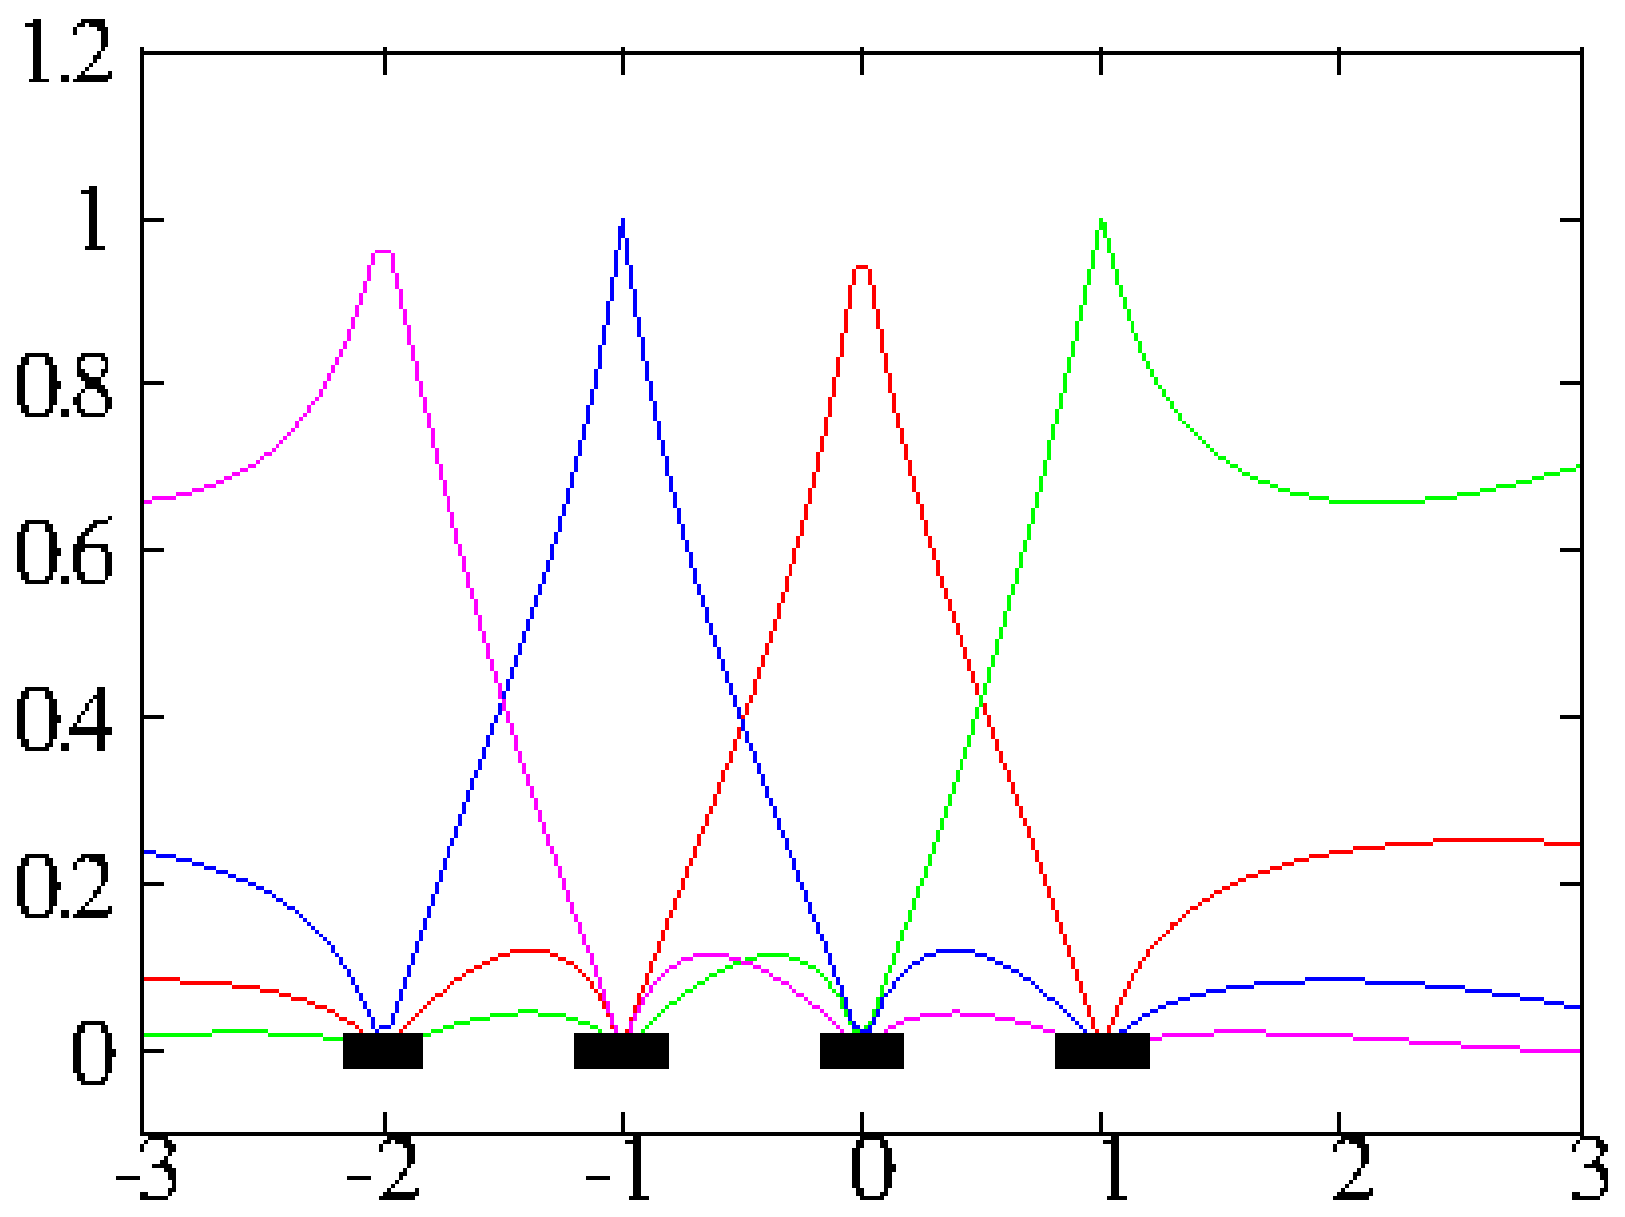
\includegraphics[scale=0.153]{./ElemShepard1.eps} &
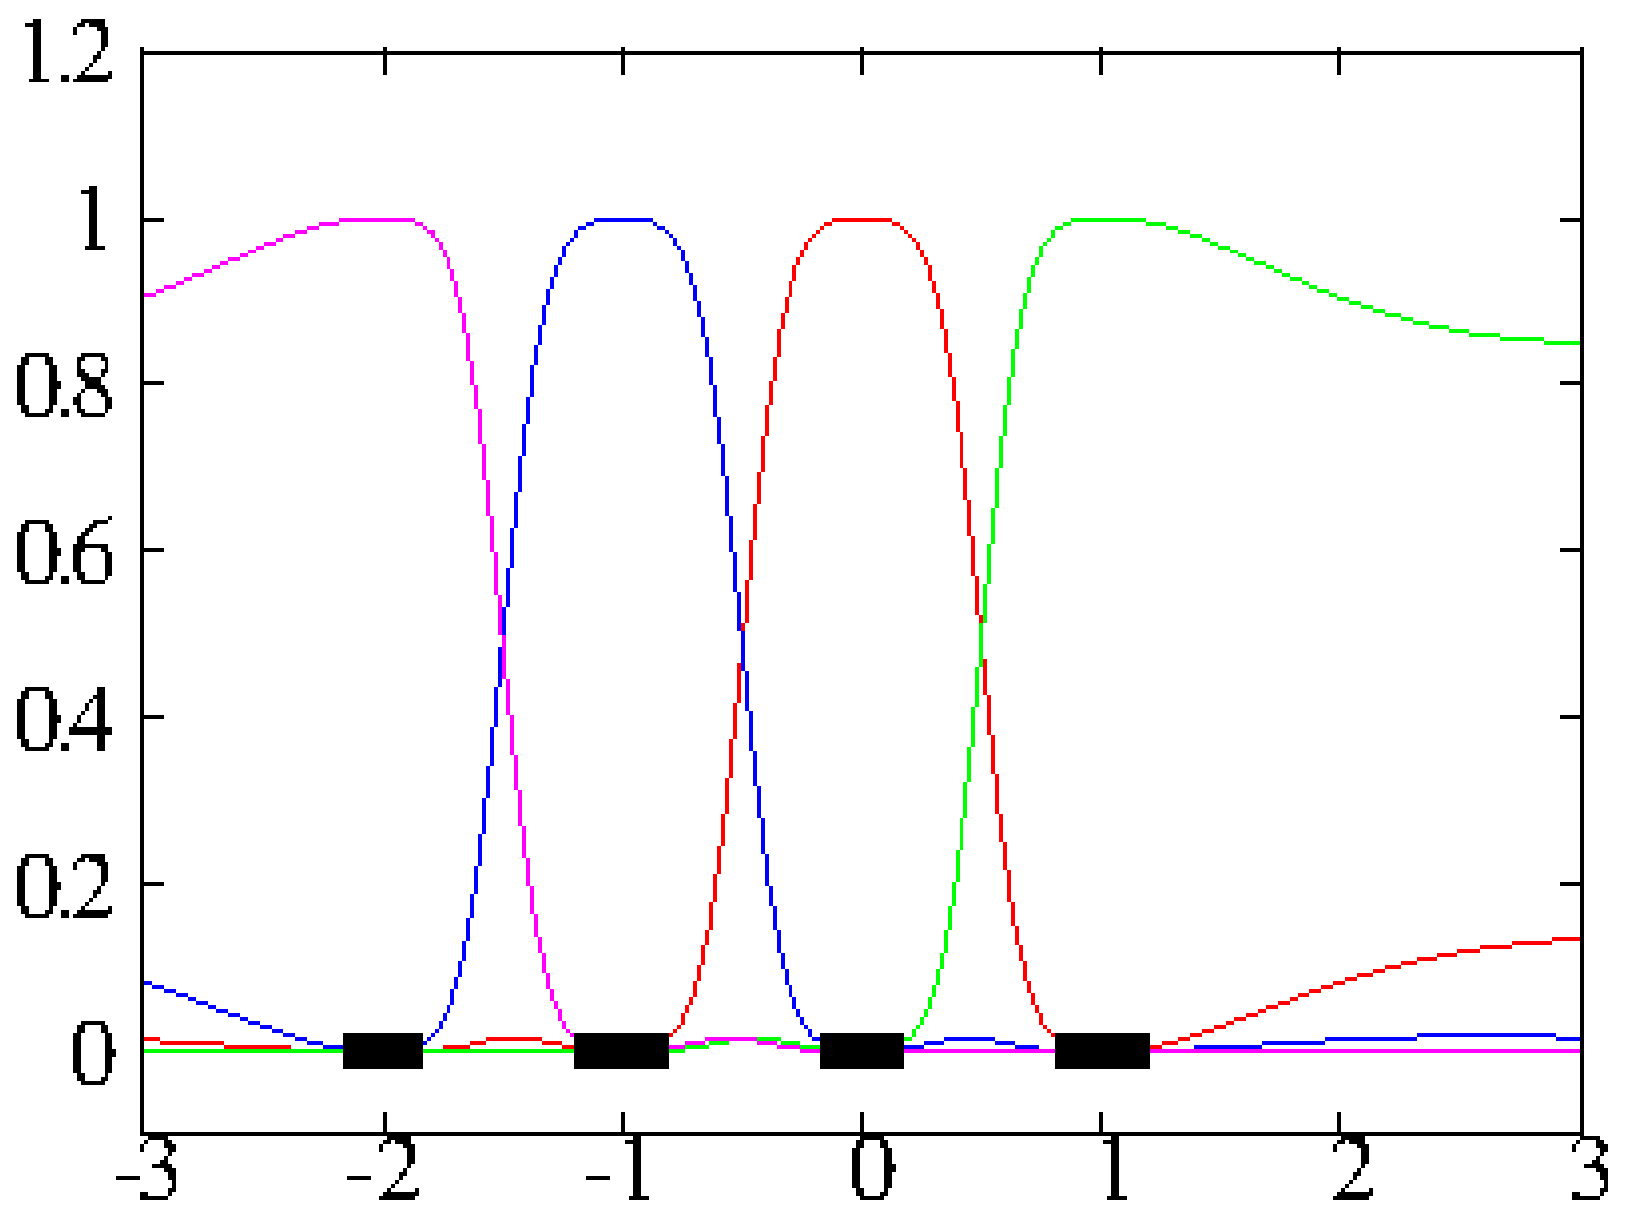
\includegraphics[scale=0.153]{./ElemShepard3.eps} \\ 
(a) & (b)\\
\end{tabular}\newline
\begin{tabular}{c}
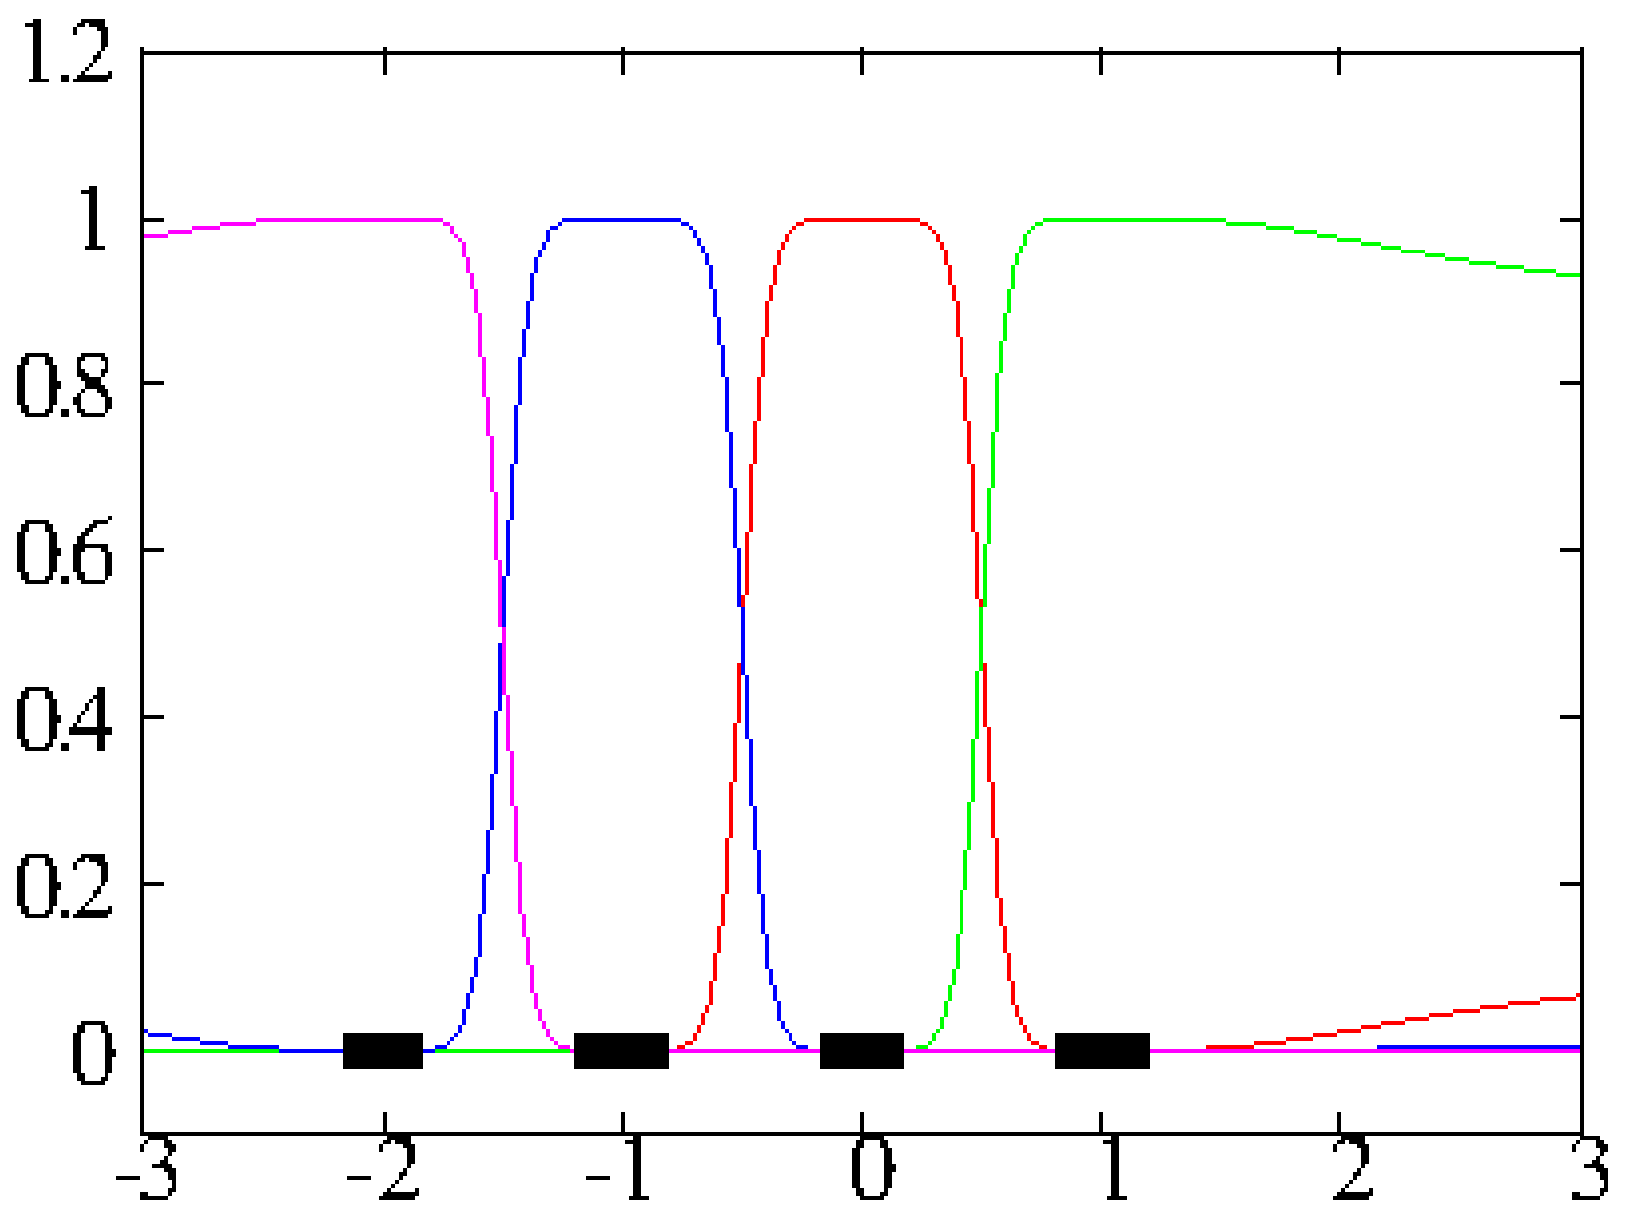
\includegraphics[scale=0.153]{./ElemShepard5.eps} \\
(c) \\
\end{tabular}
\caption{\label{fig.elemShepard}Behaviour of different Shepard bases according to three values of $k$, where the black dots stand for the center of the basis: (a) $k=1$, (b) $k=3$ and (c) $k = 5$.}
\end{figure}

Figure~\ref{fig.intShepard} depicts some interpolated functions using FEM with Shepard basis. Analogously to the behaviour of the aforementioned basis, the interpolated functions tend to become less smooth. Once more, the rectangles stand for the center of the basis.

\begin{figure}[!h]
\centering
\begin{tabular}{cc}
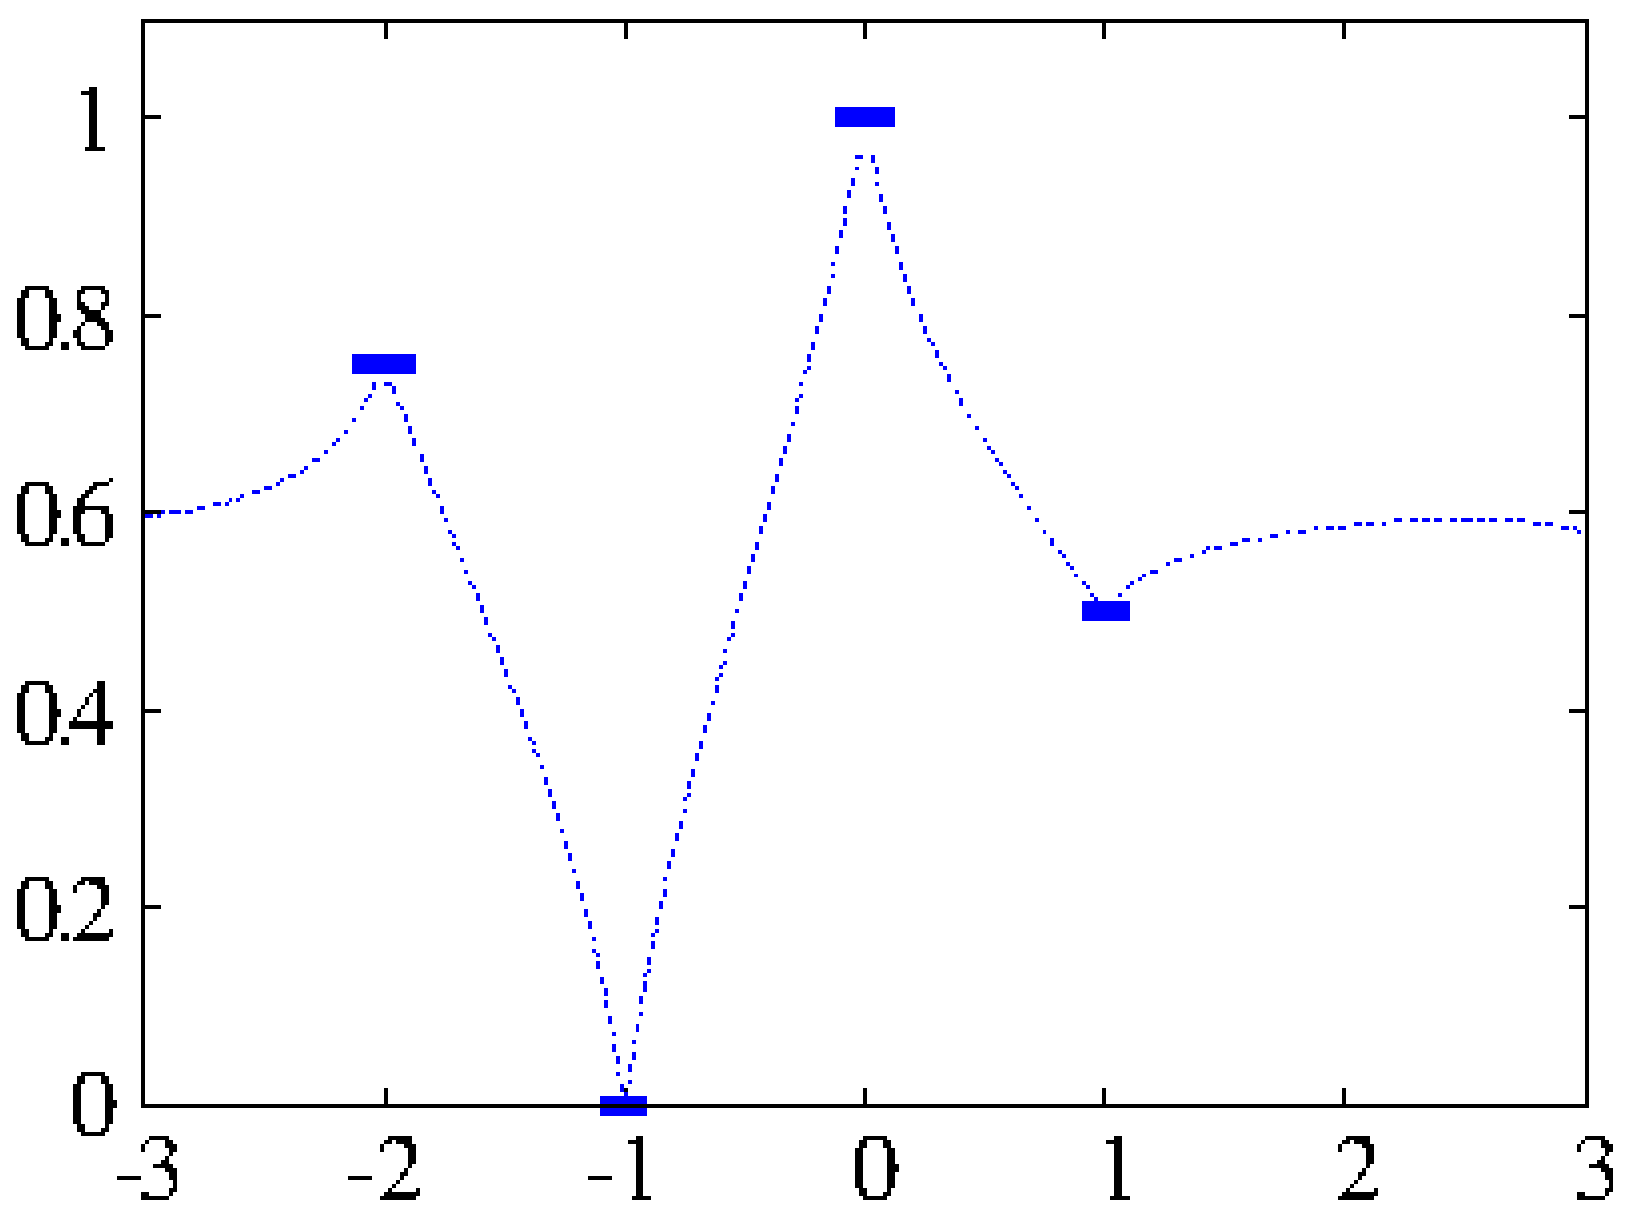
\includegraphics[scale=0.153]{./intShepard1.eps} &
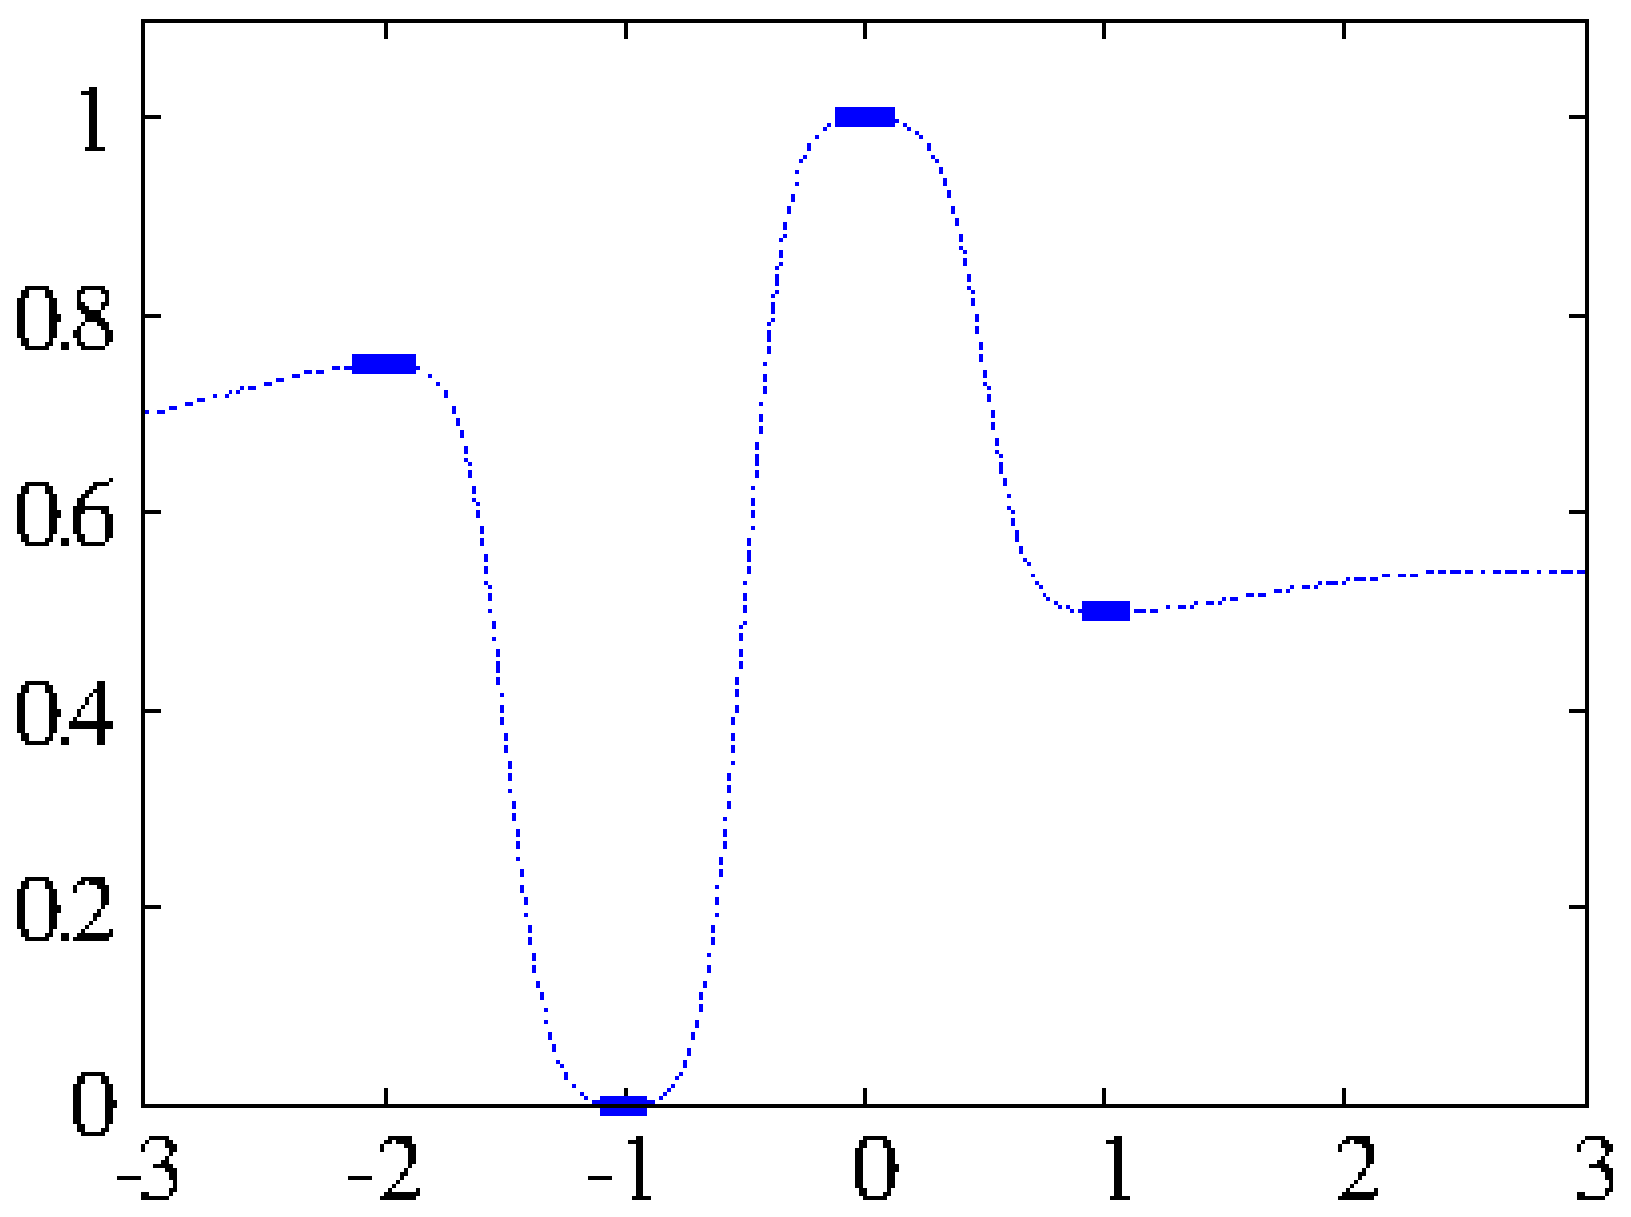
\includegraphics[scale=0.153]{./intShepard3.eps} \\ 
(a) & (b) \\
\end{tabular}
\begin{tabular}{c}
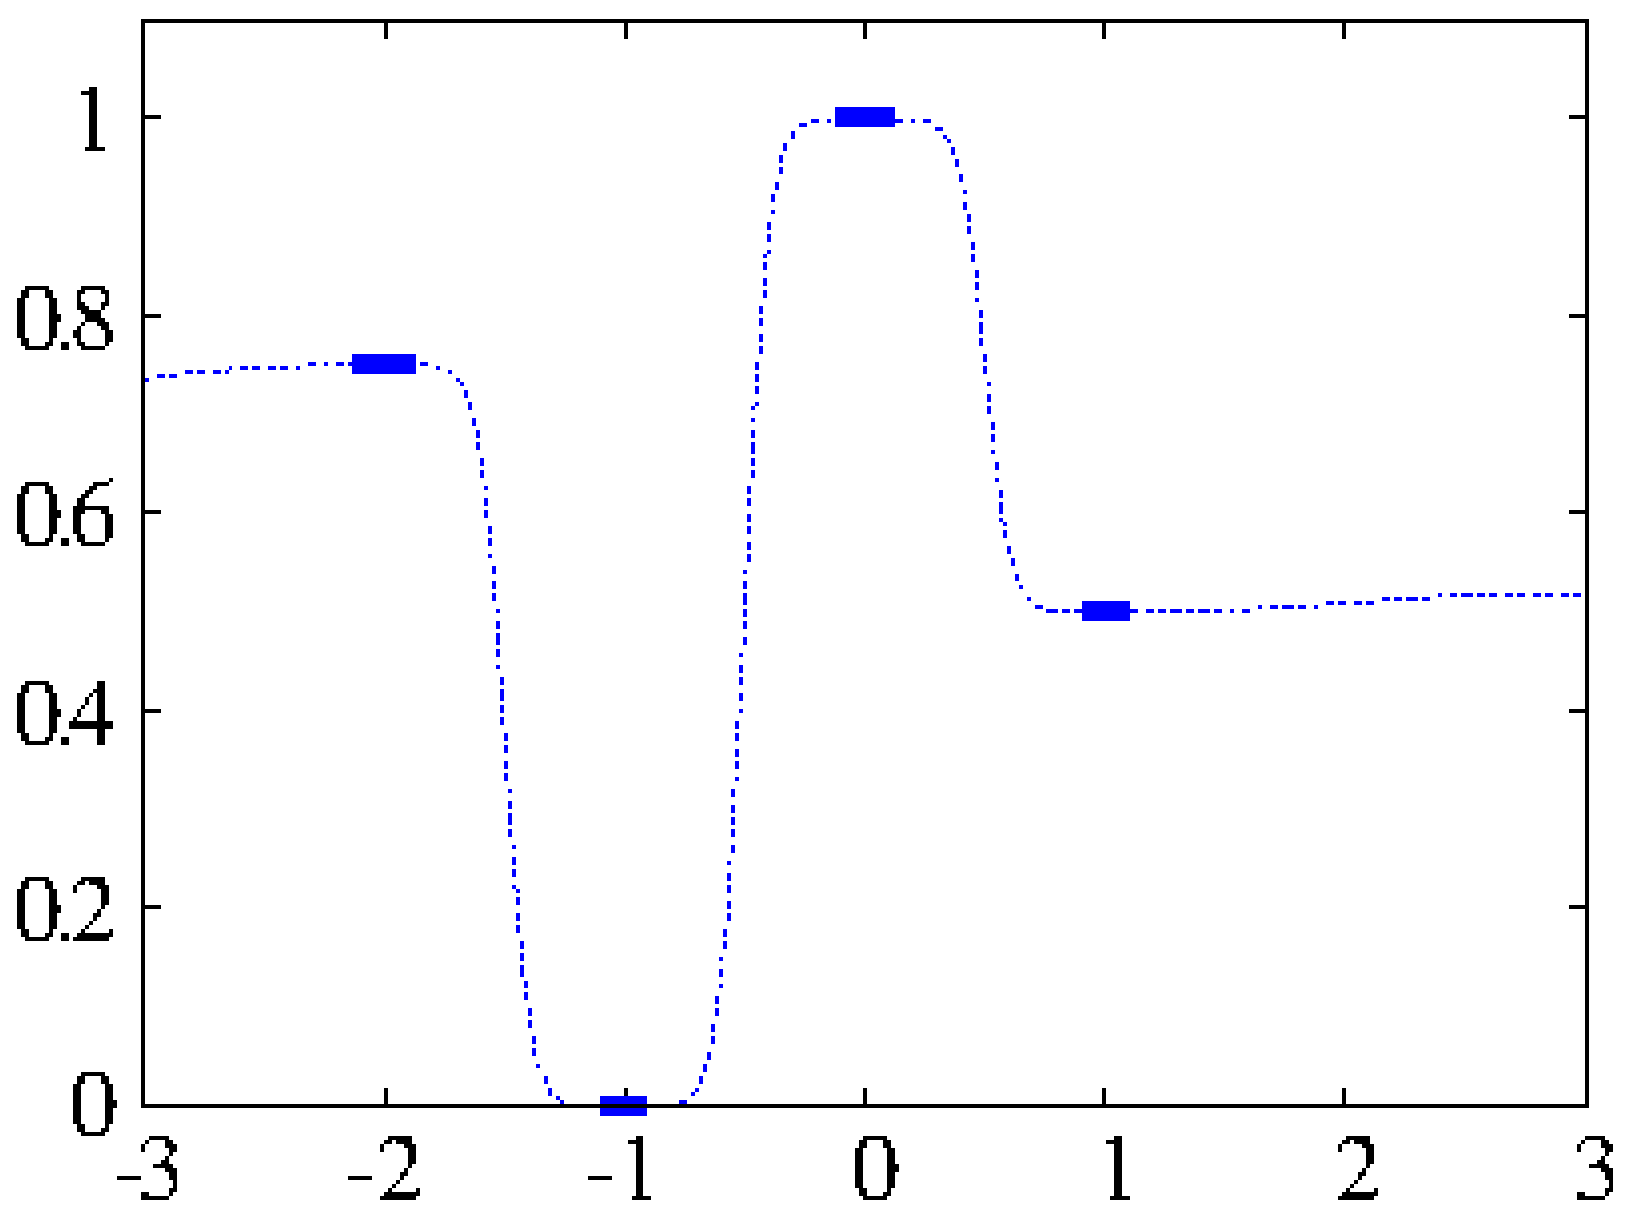
\includegraphics[scale=0.153]{./intShepard5.eps} \\
(c) \\
\end{tabular}
\caption{\label{fig.intShepard}Interpolated function using the Shepard basis for (a) $k=1$, (b) $k=3$ and (c) $k=5$. The blue rectangles represent the center of the basis and their sampled values.}
\end{figure}